\section{Introduction}
This report summarizes the work of Calvin College's senior design team 01: Team PICA during the academic year 2010-2011. Each section further breaks down a component of our system, beginning at the high-level requirements until reaching component selection. Each part of our final report relates a discussion of concepts relating to the business case for the project and the engineering design that went into producing a working prototype.

% Problem definition, from Business Plan s. 2.1
\subsection{Problem Definition}

\begin{figure}[htbp]
  \centering
  \includegraphics[width=5in]{includes/watt_hour_meter}
  \caption{Standard electric meter; photo copyright Beige Alert (Creative Commons).}
  \label{fig:mechanical_meter}
\end{figure}

Standard electric meters were developed decades ago and are still used today, despite many technological advances in the last several years. Additionally, Americans have become accustomed to having access to large amounts of data, but due to the nature of standard electric metering, data regarding the usage of power is severely limited for both the consumer and electric company. 

\begin{figure}[htbp]
  \centering
  \subfloat[MIT Power usage data.\cite{USEIA}]{\label{fig:mit_usage}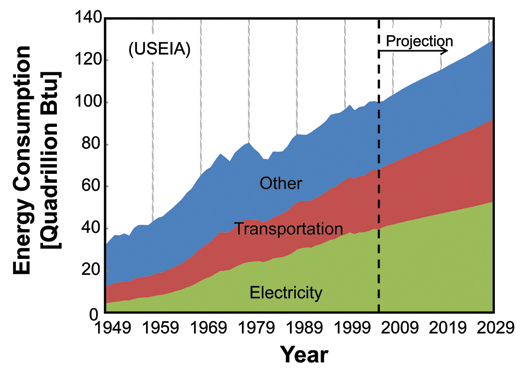
\includegraphics[width=3in]{includes/MIT_Energy_Consumption}}\ 
  \subfloat[Energy cost projections.\cite{Cost_Kilowatt}]{\label{fig:energy_cost}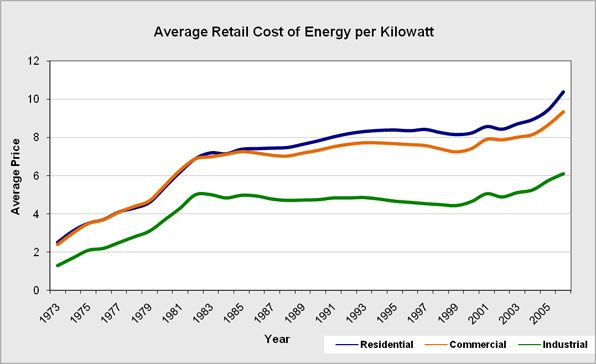
\includegraphics[width=3in]{includes/Energy_Cost}}
  \caption{Power usage and cost metrics.}
  \label{fig:power_usage_and_cost}
\end{figure}

Both usage and cost of electricity continue to increase, see figures \ref{fig:mit_usage} and \ref{fig:energy_cost} respectively, causing consumers and providers to look for ways to become more efficient. With more data about electric usage available, both parties can find inefficencies and take action as appropriate. Currently, few simple or inexpensive solutions exist, and most only address part of the whole problem, giving some information to the consumer and none to the power company or vice-versa.

%% Customer base, from business plan s. 3.5
\subsection{Customer Base}
The target market for the entire PICA system comprises both electricity
producers and electricity consumers, as set forth by the nature of the
subsystems. As the power companies supply and own the electricity meters
attached to the buildings to which they supply power, the PICA E-meter appeals
only to the market of electricity-producing companies. The other two subsystems,
the solid-state breakers and base station, target the power-consuming audience,
as the devices will assist in monitoring power flow inside the building, where
the power company has no presence. As these two markets are essentially
exclusive in both membership and interest in the PICA subsystems, the E-meter
will be able to function independently of the other consumer-targeted
subsystems, and vice versa.

\subsubsection{Power Companies} % Fixed
As power companies currently distribute the whole-building metering hardware
that determines how much energy their customer used, the E-meter clearly targets
power companies. In fact, the power companies own the power-measuring hardware
external to the buildings to while they provide power, so only they may replace
or upgrade those devices. At present, power companies send trained meter-readers
to read the data from most traditional power meters under their control. The
PICA E-meter subsystem aims to improve on this process by automatically sending
the measurements to the power company using a means and protocol selected by the
particular company. While this will require some hardware customization for each
company, the volume of company-specific production should allow the cost to
develop the design to spread into a small per-unit cost. 

The PICA E-meter subsystem also provides numerous more measures of power than
the simple spinning-dial meters. For example, the E-meter will measure the
frequency and the RMS voltage of the incoming supply lines, which help indicate
the overall quality of power delivered to the customers in the area. This
information may also help diagnose any observed issues with power delivery
without dispatching a worker to take measurements by hand. In this way, power
companies using the PICA E-meter can improve the quality of the service they
provide and can save on the labor costs associated with making a site visit. 

\subsubsection{Power Consumers}
Although the power company's customers cannot modify the metering panel
installed by the power company, they are free to modify the other power
distribution components inside their own buildings. The solid-state breakers
fall into this category, and provide previously unavailable measurements
regarding power consumption and its location within the building. However, as
these breakers will replace the pre-existing breakers inside the building, the
consumer must be convinced that using the PICA system is worth the trouble and
cost of replacing the mechanical circuit breakers with the more feature-rich
PICA breakers. To this effect, the most receptive market for the solid-state
breakers includes homeowners and building managers who are curious or concerned
about power usage inside their building. That is, the people for whom this
information can inspire a meaningful change in practice will likely become the
first adopters of the subsystem. 

The product may also gain a following as an alternative to mechanical breakers
in during the construction of a new home or building. This would likely require
that the product already have a proven history of reliability and safety, so the
previous group of cost- or environmentally-concerned individuals might have to
adopt the produce first. If the PICA solid-state breakers become an alternative
during construction, the net cost to the user will be lessened, as the
building-to-be will not have any pre-existing breakers to discard or replace. 

The base station may apply to either of these two consumer groups, as its
primary purpose is to manage and interface with the other systems. It does not
specifically require the solid-state breakers or the E-meter, but provides
little value in a building without any installed PICA systems. The base station
exists solely to manage and collect data from other PICA subsystems, as well as
format and display these measurements, so its target audience consists of power
consumers whose buildings use the E-meter, the solid-state breakers, or both.
 
\subsection{About Us}
\begin{figure}[htbp]
  \centering
  
\includegraphics[width=6in]{includes/IMG_0865}
  \caption{Team PICA left to right: Amy Ball, Kendrick Wiersma, Nathan Jen, and Avery Sterk.}
  \label{fig:team_picture}
\end{figure}
\textbf{Amy Ball}: Amy, from Wayland, Michigan, works as an intern at Johnson Controls as part of the Systems Engineering Team. She brings good communication skills, circuit-building experience, and presentation skills to the project. Originally her section was the solid-state breakers, but the team decided to use solid-state relays for the breaker purposes. After which her new task was to build all of the power supplies for the project. Additionally, she was assigned to identify a method to match outlets to breakers.


\textbf{Kendrick Wiersma}: Kendrick works as an intern at Raytheon in the Electronics Center, where he performs embedded system design and verification in \ac{VHDL}. Kendrick hails from Tucson, Arizona where he was born and raised. He brings real-world project experience and experience working with embedded hardware and software to the team. Kendrick leads the development of the E-meter, which primarily measures total power consumption, reporting data to the power company and the PICA base station.


\textbf{Nathan Jen}: Nathan, from Kentwood, Michigan, has worked at Amway on the production floor and has gained involvement with club leadership at Calvin College. He will be graduating with an Engineering degree, Electrical and Computer Concentration. He brings leadership experience and a good understanding of how smaller elements of a system fit together as a whole. After graduation, Nate has accepted a position with American Electric Power, working at the D.C. Nuclear Plant in Bridgeman, Michigan. His section of the project is the monitoring of individual circuits and some of the control logic for the breakers. 


\textbf{Avery Sterk}: Avery comes from Santa Clara, California where he worked as an intern at the SLAC National Accelerator Laboratory doing CAD design. He will be graduating with a degree in Engineering Electrical and Computer Concentration and a Math minor. He brings varied experience with software design and implementation to the project. Avery is the technical lead on the base station, especially providing the primary user interface and designing embedded software. Additionally Avery became the software lead on the E-Meter after changing the focus of the base station component of the project.
 
\subsection{About the Course}
Taken from the Calvin College course catalogue:
\begin{quote}
This course takes place over two semesters in the senior design project sequence. For the first semester course (Engineering 339), emphasis is placed on design team formation, project identification, and production of a feasibility study. Students focus on the development of task specifications in light of the norms for design and preliminary validation of the design by means of basic analysis and appropriate prototyping. Lectures focus on integration of the design process with a reformed Christian worldview, team building, and state-of-the-art technical aspects of design. Interdisciplinary projects are encouraged. Prerequisites: Concurrent registration in the seventh semester of the model program for a particular concentration or permission of the instructors; developing a Christian mind and philosophical foundations.

For the second semester in the senior design project sequence (Engineering 340), emphasis is placed on the completion of a major design project initiated in Engineering 339. This project should entail task specifications in light of the norms for design by means of engineering analysis and an appropriate prototype focused on primary functionality. A final presentation is given at the May Senior Design Night Banquet. Lectures continue to focus on integration of the design process with a Christian reformed world-view, team activity, and state-of-the art technical aspects of design.
\end{quote}